% Options for packages loaded elsewhere
\PassOptionsToPackage{unicode}{hyperref}
\PassOptionsToPackage{hyphens}{url}
\PassOptionsToPackage{dvipsnames,svgnames,x11names}{xcolor}
%
\documentclass[
  ignorenonframetext,
]{beamer}
\usepackage{pgfpages}
\setbeamertemplate{caption}[numbered]
\setbeamertemplate{caption label separator}{: }
\setbeamercolor{caption name}{fg=normal text.fg}
\beamertemplatenavigationsymbolsempty
% Prevent slide breaks in the middle of a paragraph
\widowpenalties 1 10000
\raggedbottom
\setbeamertemplate{part page}{
  \centering
  \begin{beamercolorbox}[sep=16pt,center]{part title}
    \usebeamerfont{part title}\insertpart\par
  \end{beamercolorbox}
}
\setbeamertemplate{section page}{
  \centering
  \begin{beamercolorbox}[sep=12pt,center]{section title}
    \usebeamerfont{section title}\insertsection\par
  \end{beamercolorbox}
}
\setbeamertemplate{subsection page}{
  \centering
  \begin{beamercolorbox}[sep=8pt,center]{subsection title}
    \usebeamerfont{subsection title}\insertsubsection\par
  \end{beamercolorbox}
}
\AtBeginPart{
  \frame{\partpage}
}
\AtBeginSection{
  \ifbibliography
  \else
    \frame{\sectionpage}
  \fi
}
\AtBeginSubsection{
  \frame{\subsectionpage}
}

\usepackage{amsmath,amssymb}
\usepackage{iftex}
\ifPDFTeX
  \usepackage[T1]{fontenc}
  \usepackage[utf8]{inputenc}
  \usepackage{textcomp} % provide euro and other symbols
\else % if luatex or xetex
  \usepackage{unicode-math}
  \defaultfontfeatures{Scale=MatchLowercase}
  \defaultfontfeatures[\rmfamily]{Ligatures=TeX,Scale=1}
\fi
\usepackage{lmodern}
\usetheme[]{Dresden}
\usefonttheme{structurebold}
\ifPDFTeX\else  
    % xetex/luatex font selection
\fi
% Use upquote if available, for straight quotes in verbatim environments
\IfFileExists{upquote.sty}{\usepackage{upquote}}{}
\IfFileExists{microtype.sty}{% use microtype if available
  \usepackage[]{microtype}
  \UseMicrotypeSet[protrusion]{basicmath} % disable protrusion for tt fonts
}{}
\makeatletter
\@ifundefined{KOMAClassName}{% if non-KOMA class
  \IfFileExists{parskip.sty}{%
    \usepackage{parskip}
  }{% else
    \setlength{\parindent}{0pt}
    \setlength{\parskip}{6pt plus 2pt minus 1pt}}
}{% if KOMA class
  \KOMAoptions{parskip=half}}
\makeatother
\usepackage{xcolor}
\newif\ifbibliography
\setlength{\emergencystretch}{3em} % prevent overfull lines
\setcounter{secnumdepth}{-\maxdimen} % remove section numbering


\providecommand{\tightlist}{%
  \setlength{\itemsep}{0pt}\setlength{\parskip}{0pt}}\usepackage{longtable,booktabs,array}
\usepackage{calc} % for calculating minipage widths
\usepackage{caption}
% Make caption package work with longtable
\makeatletter
\def\fnum@table{\tablename~\thetable}
\makeatother
\usepackage{graphicx}
\makeatletter
\newsavebox\pandoc@box
\newcommand*\pandocbounded[1]{% scales image to fit in text height/width
  \sbox\pandoc@box{#1}%
  \Gscale@div\@tempa{\textheight}{\dimexpr\ht\pandoc@box+\dp\pandoc@box\relax}%
  \Gscale@div\@tempb{\linewidth}{\wd\pandoc@box}%
  \ifdim\@tempb\p@<\@tempa\p@\let\@tempa\@tempb\fi% select the smaller of both
  \ifdim\@tempa\p@<\p@\scalebox{\@tempa}{\usebox\pandoc@box}%
  \else\usebox{\pandoc@box}%
  \fi%
}
% Set default figure placement to htbp
\def\fps@figure{htbp}
\makeatother
% definitions for citeproc citations
\NewDocumentCommand\citeproctext{}{}
\NewDocumentCommand\citeproc{mm}{%
  \begingroup\def\citeproctext{#2}\cite{#1}\endgroup}
\makeatletter
 % allow citations to break across lines
 \let\@cite@ofmt\@firstofone
 % avoid brackets around text for \cite:
 \def\@biblabel#1{}
 \def\@cite#1#2{{#1\if@tempswa , #2\fi}}
\makeatother
\newlength{\cslhangindent}
\setlength{\cslhangindent}{1.5em}
\newlength{\csllabelwidth}
\setlength{\csllabelwidth}{3em}
\newenvironment{CSLReferences}[2] % #1 hanging-indent, #2 entry-spacing
 {\begin{list}{}{%
  \setlength{\itemindent}{0pt}
  \setlength{\leftmargin}{0pt}
  \setlength{\parsep}{0pt}
  % turn on hanging indent if param 1 is 1
  \ifodd #1
   \setlength{\leftmargin}{\cslhangindent}
   \setlength{\itemindent}{-1\cslhangindent}
  \fi
  % set entry spacing
  \setlength{\itemsep}{#2\baselineskip}}}
 {\end{list}}
\usepackage{calc}
\newcommand{\CSLBlock}[1]{\hfill\break\parbox[t]{\linewidth}{\strut\ignorespaces#1\strut}}
\newcommand{\CSLLeftMargin}[1]{\parbox[t]{\csllabelwidth}{\strut#1\strut}}
\newcommand{\CSLRightInline}[1]{\parbox[t]{\linewidth - \csllabelwidth}{\strut#1\strut}}
\newcommand{\CSLIndent}[1]{\hspace{\cslhangindent}#1}

%% add lmu logo to title slide
\titlegraphic{
\includegraphics[width=0.33\textwidth]{extra/lmu-logo.png}}

%% modify color template to lmu-inspired one
\definecolor{lmugreen}{RGB}{0,136,58}
\setbeamercolor*{palette primary}{bg=lmugreen!10}
\setbeamercolor{title}{bg=lmugreen!10, fg=lmugreen}
\setbeamercolor{item}{fg=lmugreen}
\setbeamercolor{enumerate item}{fg=lmugreen}
\setbeamercolor{structure}{fg=lmugreen}
\setbeamercolor{titlelike}{parent=palette primary,fg=lmugreen}
\setbeamercolor{bibliography entry author}{fg=black}

%% modify beamer template to have slide number on footer
\setbeamertemplate{footline}%{miniframes theme}
{%
  \begin{beamercolorbox}[colsep=1.5pt]{upper separation line foot}
  \end{beamercolorbox}
  \begin{beamercolorbox}[ht=2.5ex,dp=1.125ex,%
    leftskip=.3cm,rightskip=.3cm plus1fil]{author in head/foot}%
    \leavevmode{\usebeamerfont{author in head/foot}\insertshortauthor}%
    \hfill%
    {\usebeamerfont{institute in head/foot}\usebeamercolor[fg]{institute in head/foot}\insertshortinstitute}%
  \end{beamercolorbox}%
  \begin{beamercolorbox}[ht=2.5ex,dp=1.125ex,%
    leftskip=.3cm,rightskip=.3cm plus1fil]{title in head/foot}%
    {\usebeamerfont{title in head/foot}\insertshorttitle} \hfill     \insertframenumber/\inserttotalframenumber%
  \end{beamercolorbox}%
  \begin{beamercolorbox}[colsep=1.5pt]{lower separation line foot}
  \end{beamercolorbox}
}

%% disable colored links for header/footer
\makeatletter
\newcommand\disablecolorlinks{\def\HyColor@UseColor##1{}}
\makeatother
\addtobeamertemplate{headline}{\disablecolorlinks{}}{}
\addtobeamertemplate{footline}{\disablecolorlinks{}}{}
\makeatletter
\@ifpackageloaded{caption}{}{\usepackage{caption}}
\AtBeginDocument{%
\ifdefined\contentsname
  \renewcommand*\contentsname{Table of contents}
\else
  \newcommand\contentsname{Table of contents}
\fi
\ifdefined\listfigurename
  \renewcommand*\listfigurename{List of Figures}
\else
  \newcommand\listfigurename{List of Figures}
\fi
\ifdefined\listtablename
  \renewcommand*\listtablename{List of Tables}
\else
  \newcommand\listtablename{List of Tables}
\fi
\ifdefined\figurename
  \renewcommand*\figurename{Figure}
\else
  \newcommand\figurename{Figure}
\fi
\ifdefined\tablename
  \renewcommand*\tablename{Table}
\else
  \newcommand\tablename{Table}
\fi
}
\@ifpackageloaded{float}{}{\usepackage{float}}
\floatstyle{ruled}
\@ifundefined{c@chapter}{\newfloat{codelisting}{h}{lop}}{\newfloat{codelisting}{h}{lop}[chapter]}
\floatname{codelisting}{Listing}
\newcommand*\listoflistings{\listof{codelisting}{List of Listings}}
\makeatother
\makeatletter
\makeatother
\makeatletter
\@ifpackageloaded{caption}{}{\usepackage{caption}}
\@ifpackageloaded{subcaption}{}{\usepackage{subcaption}}
\makeatother

\usepackage{bookmark}

\IfFileExists{xurl.sty}{\usepackage{xurl}}{} % add URL line breaks if available
\urlstyle{same} % disable monospaced font for URLs
\hypersetup{
  pdftitle={Generalization Bounds},
  pdfauthor={Matteo Mazzarelli},
  colorlinks=true,
  linkcolor={lmugreen},
  filecolor={Maroon},
  citecolor={Blue},
  urlcolor={Blue},
  pdfcreator={LaTeX via pandoc}}


\title{Generalization Bounds}
\subtitle{Theoretical Foundations of Deep Learning}
\author{Matteo Mazzarelli}
\date{December 17, 2024}

\begin{document}
\frame{\titlepage}


\section{Introduction}\label{introduction}

\begin{frame}{Why Study Generalization?}
\phantomsection\label{why-study-generalization}
\begin{itemize}
\tightlist
\item
  \textbf{Core Question}: How can models trained on limited data perform
  reliably on unseen scenarios?
\item
  \textbf{Generalization} is a fundamental goal in machine learning:
  ensuring models extend their learned patterns to new, unseen data.
\item
  A poorly generalized model risks:

  \begin{itemize}
  \tightlist
  \item
    \textbf{Overfitting}: Performing well on training data but poorly on
    unseen data.
  \item
    \textbf{Underfitting}: Failing to capture the underlying patterns of
    the data.
  \end{itemize}
\end{itemize}
\end{frame}

\begin{frame}{Defining Generalization}
\phantomsection\label{defining-generalization}
\begin{itemize}
\tightlist
\item
  \textbf{Supervised Learning}: Learn a function \(f\!\!: X \to Y\) from
  labeled training data.
\item
  \textbf{Challenge}: The learned function must perform well
  \emph{beyond} the training set.
\item
  \textbf{Evaluation}: We assess generalization by comparing model
  performance on training data versus a separate \emph{testing} dataset
  representing unseen scenarios. This helps us understand how well the
  model will perform in the real world.
\end{itemize}
\end{frame}

\section{Overfitting}\label{overfitting}

\begin{frame}{Demonstrating Overfitting}
\phantomsection\label{demonstrating-overfitting}
\begin{itemize}
\tightlist
\item
  \textbf{Objective}:

  \begin{itemize}
  \tightlist
  \item
    Show how increasing model complexity (polynomial degree) leads to
    overfitting.
  \end{itemize}
\item
  \textbf{Dataset}:

  \begin{itemize}
  \tightlist
  \item
    Using the scikit-learn \textbf{Diabetes} dataset with a single
    feature (BMI) and a quantitative response variable indicating
    disease progression
    (Target)\textsuperscript{{[}\citeproc{ref-sklearndiabetes11}{1}{]}}.
  \end{itemize}
\item
  \textbf{Approach}:

  \begin{enumerate}
  \tightlist
  \item
    Fit polynomial regression models of varying degrees.
  \item
    Visualize polynomial fits on the training data.
  \item
    Examine the fits' residuals to see how errors behave.
  \item
    Plot training vs.~test errors to highlight overfitting.
  \end{enumerate}
\end{itemize}
\end{frame}

\begin{frame}
\begin{figure}[H]

{\centering \pandocbounded{\includegraphics[keepaspectratio]{generalization-bounds_presentation_files/figure-beamer/cell-2-output-1.pdf}}

}

\caption{Overfitting Phenomenon in Polynomial Regression}

\end{figure}%
\end{frame}

\begin{frame}{Double Descent}
\phantomsection\label{double-descent}
\begin{itemize}
\tightlist
\item
  Modern machine learning introduces a fascinating twist: \textbf{Double
  Descent}, where increasing model complexity can lead to improved
  generalization after an initial overfitting phase.
\end{itemize}

\begin{figure}[H]

{\centering 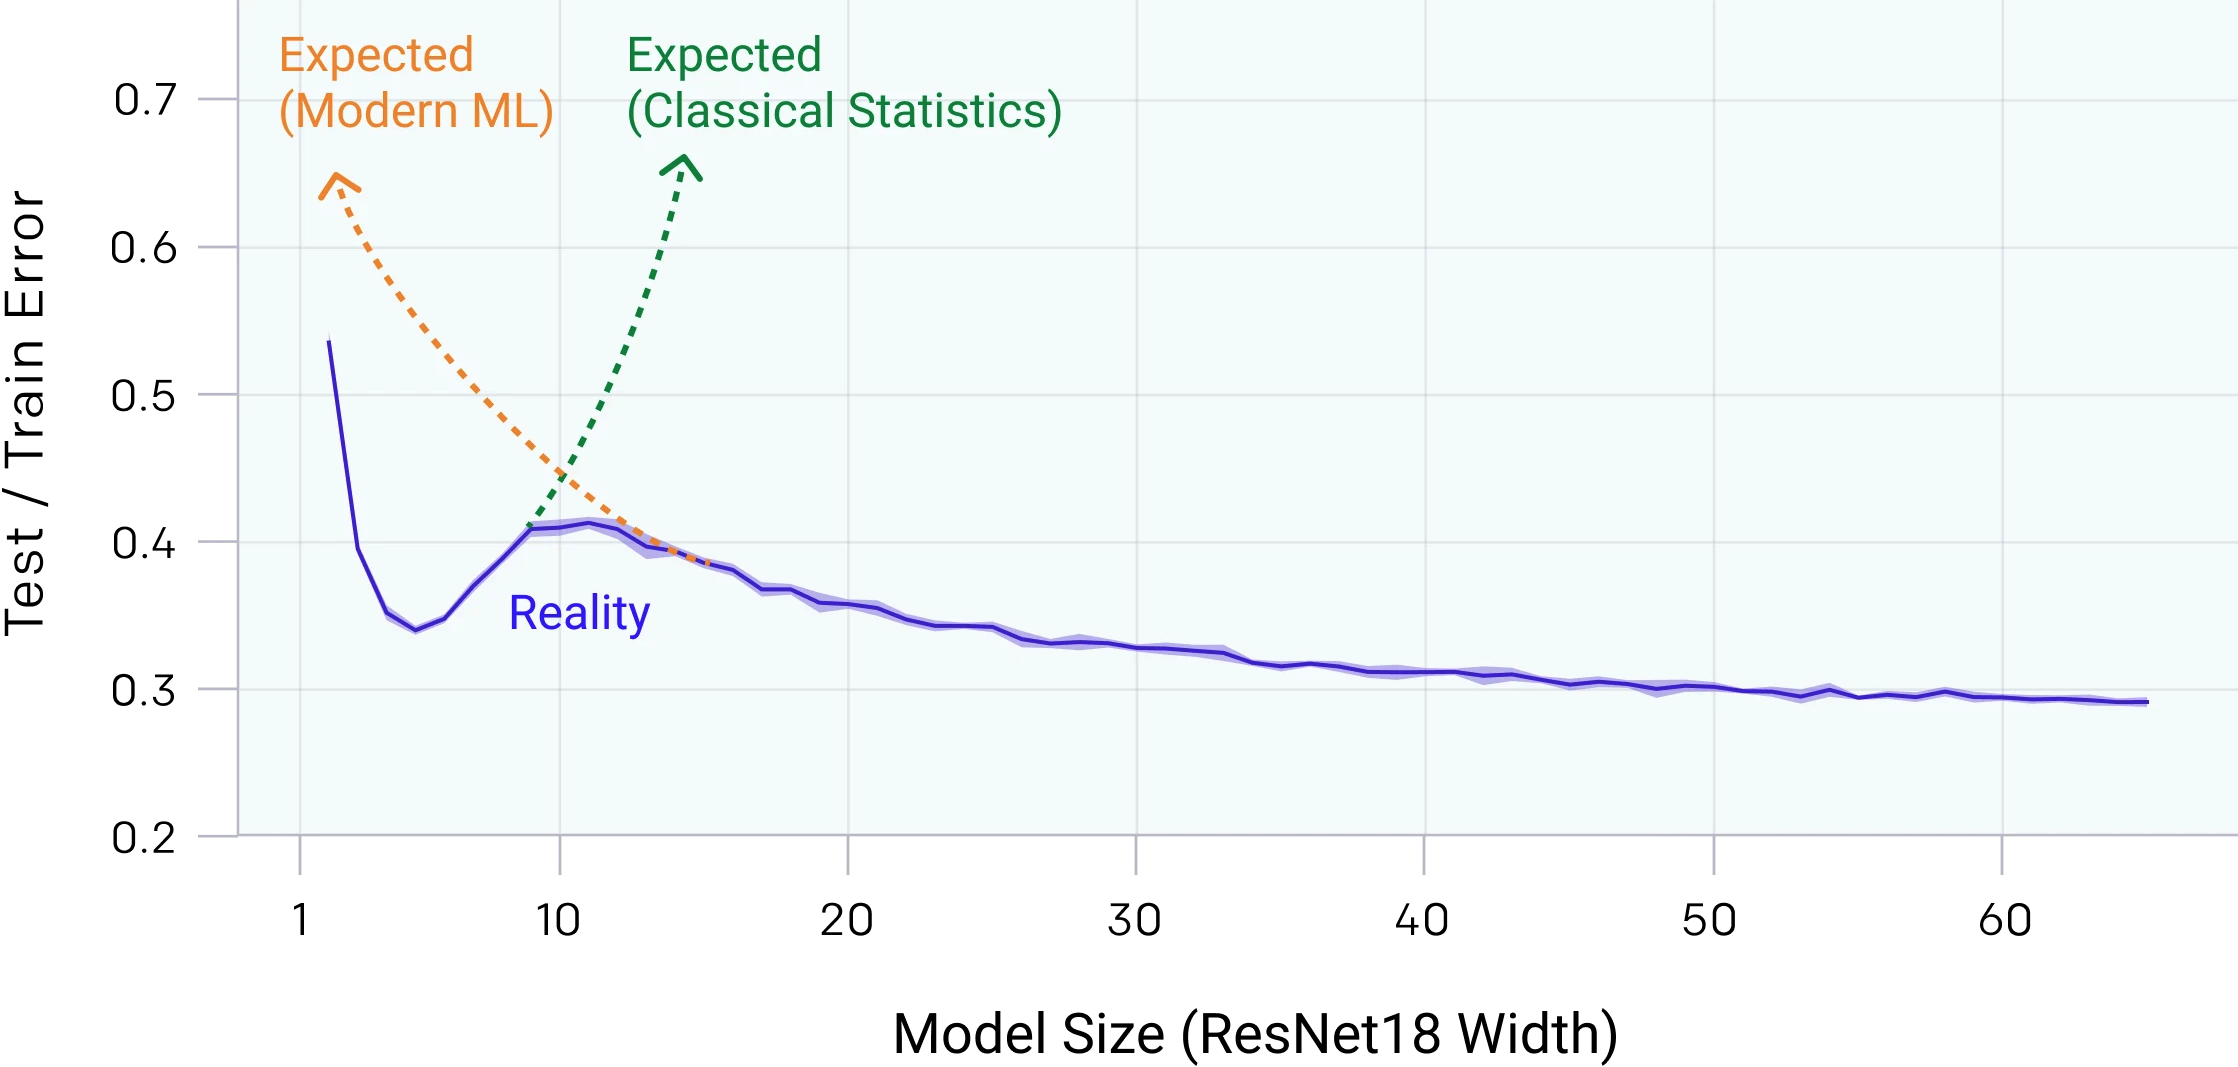
\includegraphics[width=0.86\linewidth,height=\textheight,keepaspectratio]{extra/double_descent.png}

}

\caption{Double Descent phenomenon in a Residual Neural
Network\textsuperscript{{[}\citeproc{ref-nakkiran19}{2}{]}}}

\end{figure}%
\end{frame}

\section{Classical Bounds}\label{classical-bounds}

\begin{frame}{Generalization Bounds}
\phantomsection\label{generalization-bounds}
\begin{itemize}
\tightlist
\item
  \textbf{Goal}: Predict a model's performance on \textbf{unseen data}.
\item
  \textbf{Generalization Bounds} provide theoretical guarantees,
  linking:

  \begin{itemize}
  \tightlist
  \item
    \textbf{Generalization Error}: Error on unseen data.
  \item
    \textbf{Empirical Risk}: Error on training data.
  \item
    \textbf{Model Complexity}: Model's flexibility.
  \end{itemize}
\item
  \textbf{Why They Matter}: They help understand the trade-offs between:

  \begin{itemize}
  \tightlist
  \item
    \textbf{Accuracy}: How well the model fits the data.
  \item
    \textbf{Complexity}: Ability to model intricate patterns.
  \item
    \textbf{Data Size}: Amount of data needed for reliable learning.
  \end{itemize}
\end{itemize}
\end{frame}

\begin{frame}{Hoeffding's Inequality}
\phantomsection\label{hoeffdings-inequality}
\begin{itemize}
\tightlist
\item
  \textbf{What it is}: A probabilistic tool that helps estimate how well
  a model will generalize.
\item
  \textbf{Focus}: Quantifies the difference between \textbf{empirical
  risk} (training error) and \textbf{generalization error} (true error)
  for a \emph{single, fixed model}.
\end{itemize}
\end{frame}

\begin{frame}{Hoeffding's Inequality: The Math}
\phantomsection\label{hoeffdings-inequality-the-math}
\begin{itemize}
\tightlist
\item
  \textbf{Expression}\textsuperscript{{[}\citeproc{ref-mohri12}{3}{]}}:
  \[
  P(|R(h) - R_{\text{emp}}(h)| > \varepsilon) \leq 2 \exp(-2n\varepsilon^2)
  \]
\item
  \textbf{Breakdown}:

  \begin{itemize}
  \tightlist
  \item
    \(R(h)\): The \textbf{true risk} of hypothesis \(h\), defined as the
    expected loss over the data distribution:
    \(R(h) = \mathbb{E}_{x,y \sim D}[\ell(h(x), y)]\).
  \item
    \(R_{\text{emp}}(h)\): The \textbf{empirical risk} of hypothesis
    \(h\), defined as the average loss over the training dataset \(S\)
    of size \(n\):
    \(R_{\text{emp}}(h) = \frac{1}{n} \sum_{i=1}^{n} \ell(h(x_i), y_i)\).
  \item
    \(\varepsilon\): Error tolerance.
  \item
    \(n\): Dataset size.
  \end{itemize}
\end{itemize}
\end{frame}

\begin{frame}{Hoeffding's Inequality: Convergence}
\phantomsection\label{hoeffdings-inequality-convergence}
\begin{itemize}
\tightlist
\item
  \textbf{Rate of Convergence}: Simulating biased coin flips to show the
  rate at which sample mean approaches the true probability.
\item
  \textbf{Hoeffding's Bound}, derived from the
  \(\exp(-2n\varepsilon^2)\) term, shows \textbf{faster convergence} as
  \(n\) increases.
\end{itemize}

\begin{figure}[H]

{\centering \pandocbounded{\includegraphics[keepaspectratio]{generalization-bounds_presentation_files/figure-beamer/cell-3-output-1.pdf}}

}

\caption{Convergence to True Probability with Hoeffding Bounds}

\end{figure}%
\end{frame}

\begin{frame}{Hoeffding's Inequality: Interpretation}
\phantomsection\label{hoeffdings-inequality-interpretation}
\begin{itemize}
\tightlist
\item
  The probability of a large difference between the true risk
  (generalization error) and the empirical risk (training error)
  decreases \textbf{exponentially} with:

  \begin{itemize}
  \tightlist
  \item
    \textbf{Larger datasets} (\(n\)).
  \item
    \textbf{Smaller error tolerance} (\(\varepsilon\)).
  \end{itemize}
\item
  \textbf{Note}: Hoeffding's inequality applies more generally to the
  difference between the sample average and the expectation of any
  bounded random variable. We have shown a special application of the
  inequality.
\item
  \textbf{Limitations}: We usually pick the best model from many, not
  just one. Hoeffding doesn't account for how complex the model class
  is.
\end{itemize}
\end{frame}

\begin{frame}{Union Bound}
\phantomsection\label{union-bound}
\begin{itemize}
\tightlist
\item
  \textbf{What it does}: Extends bounds like Hoeffding's to work when
  choosing from \textbf{many models} (a hypothesis space
  \(\mathcal{H}\)).
\item
  \textbf{Main Idea}: Considers the chance that \emph{at least one}
  model in \(\mathcal{H}\) has a large difference between training and
  true error.
\end{itemize}
\end{frame}

\begin{frame}{Union Bound: The Math}
\phantomsection\label{union-bound-the-math}
\begin{itemize}
\tightlist
\item
  \textbf{Expression}\textsuperscript{{[}\citeproc{ref-samir16}{4}{]}}:
  \[
  P\left(\sup_{h \in \mathcal{H}} |R(h) - R_{\text{emp}}(h)| > \epsilon \right) \leq \sum_{h \in \mathcal{H}} P\left(|R(h) - R_{\text{emp}}(h)| > \epsilon \right)
  \]
\item
  \textbf{Breakdown}:

  \begin{itemize}
  \tightlist
  \item
    \(R(h)\): True risk (expected loss).
  \item
    \(R_{\text{emp}}(h)\): Empirical risk (average training loss).
  \item
    \(\sup_{h \in \mathcal{H}}\): Account for the worst-case scenario
    across all hypotheses, considering the largest deviation between
    true and empirical risk.
  \item
    \(\sum_{h \in \mathcal{H}}\): Sums up probabilities of large error
    differences for each model in the hypothesis space \(\mathcal{H}\).
  \end{itemize}
\end{itemize}
\end{frame}

\begin{frame}{Union Bound: Interpretation}
\phantomsection\label{union-bound-interpretation}
\begin{itemize}
\tightlist
\item
  \textbf{Larger Model Space}: The more models we consider, the looser
  the bound becomes.
\end{itemize}

\begin{longtable}[]{@{}lll@{}}
\caption{Trade-off: Hypothesis Space vs.~Bound \&
Capacity}\tabularnewline
\toprule\noalign{}
\textbf{Hypothesis Space Size} & \textbf{Bound} & \textbf{Model
Capacity} \\
\midrule\noalign{}
\endfirsthead
\toprule\noalign{}
\textbf{Hypothesis Space Size} & \textbf{Bound} & \textbf{Model
Capacity} \\
\midrule\noalign{}
\endhead
Small & Tighter & Limited \\
Large & Looser & Higher \\
\bottomrule\noalign{}
\end{longtable}
\end{frame}

\begin{frame}{Moving Forward}
\phantomsection\label{moving-forward}
\begin{itemize}
\tightlist
\item
  \textbf{Challenge}: Real-world model spaces are often infinite or too
  large.
\item
  \textbf{Solution}: We need ways to measure model complexity that go
  beyond counting.
\item
  \textbf{Next}: Exploring \textbf{complexity measures} for more
  practical generalization bounds.
\end{itemize}
\end{frame}

\section{Advanced Bounds}\label{advanced-bounds}

\begin{frame}{Why Advanced Bounds?}
\phantomsection\label{why-advanced-bounds}
\begin{itemize}
\tightlist
\item
  \textbf{Classical Bounds} give us a good starting point, but they can
  be loose.
\item
  \textbf{Goal}: Tighter bounds that better reflect real-world
  performance.
\item
  \textbf{How?}: By measuring model complexity in more sophisticated
  ways.
\end{itemize}
\end{frame}

\begin{frame}{VC Dimension}
\phantomsection\label{vc-dimension}
\begin{itemize}
\tightlist
\item
  \textbf{Growth Function} (\(\Pi_{\mathcal{H}}(n)\)): How many ways can
  a model class (\(\mathcal{H}\)) label \emph{n} data points?

  \begin{itemize}
  \tightlist
  \item
    More ways = more complex.
  \item
    For small \emph{n}, \(\Pi_{\mathcal{H}}(n)=2^n\).
  \end{itemize}
\item
  \textbf{Shattering}: A model class \emph{shatters} a dataset if it can
  label it in \emph{every possible way}.
\end{itemize}
\end{frame}

\begin{frame}{VC Dimension: Definition}
\phantomsection\label{vc-dimension-definition}
\begin{itemize}
\tightlist
\item
  \textbf{VC Dimension (\(d_{\text{VC}}\))}: The size of the
  \emph{largest} dataset a model class can shatter.
\item
  \textbf{Example}: Linear classifiers in 2D have \(d_{\text{VC}} = 3\).
  They can shatter 3 points but not 4 (in all configurations).
\end{itemize}

\begin{figure}[H]

{\centering \pandocbounded{\includegraphics[keepaspectratio]{generalization-bounds_presentation_files/figure-beamer/cell-4-output-1.pdf}}

}

\caption{VC Dimension of Linear Classifiers in 2D}

\end{figure}%

\begin{itemize}
\tightlist
\item
  \textbf{Intuition}: Higher \(d_{\text{VC}}\) = more complex model.
\end{itemize}
\end{frame}

\begin{frame}{VC Generalization Bound: The Math}
\phantomsection\label{vc-generalization-bound-the-math}
\begin{itemize}
\tightlist
\item
  \textbf{Expression}\textsuperscript{{[}\citeproc{ref-vapnik95}{5}{]}}:
  \[
  R(h) \leq R_{\text{emp}}(h) + \sqrt{\frac{8 d_{\text{VC}} \left(\ln\left(\frac{2n}{d_{\text{VC}}}\right) + 1\right) + 8 \ln\left(\frac{4}{\delta}\right)}{n}}
  \]
\item
  \textbf{Breakdown}:

  \begin{itemize}
  \tightlist
  \item
    \(R(h)\): True risk (expected loss).
  \item
    \(R_{\text{emp}}(h)\): Empirical risk (average training loss).
  \item
    \(d_{\text{VC}}\): VC dimension.
  \item
    \(n\): Dataset size.
  \item
    \(\delta\): Confidence parameter.
  \end{itemize}
\end{itemize}
\end{frame}

\begin{frame}{VC Generalization Bound: Interpretation}
\phantomsection\label{vc-generalization-bound-interpretation}
\begin{itemize}
\tightlist
\item
  \textbf{Higher VC Dimension}:

  \begin{itemize}
  \tightlist
  \item
    More complex model, looser bound, higher risk of overfitting.
  \end{itemize}
\item
  \textbf{Larger Dataset}:

  \begin{itemize}
  \tightlist
  \item
    Tighter bound, better generalization.
  \end{itemize}
\end{itemize}

\begin{figure}[H]

{\centering \pandocbounded{\includegraphics[keepaspectratio]{generalization-bounds_presentation_files/figure-beamer/cell-5-output-1.pdf}}

}

\caption{Approximation of the VC Generalization Bound}

\end{figure}%
\end{frame}

\begin{frame}{Distribution-Based Bounds}
\phantomsection\label{distribution-based-bounds}
\begin{itemize}
\tightlist
\item
  \textbf{VC theory} often considers the \emph{worst-case} scenario.
\item
  \textbf{New Idea}: Use information about the \textbf{data
  distribution} for tighter bounds.
\item
  \textbf{Benefit}: More realistic bounds reflecting real-world
  performance.
\end{itemize}
\end{frame}

\begin{frame}{Support Vector Machines}
\phantomsection\label{support-vector-machines}
\begin{itemize}
\tightlist
\item
  \textbf{Example}: Support Vector Machines (SVMs).

  \begin{itemize}
  \tightlist
  \item
    \textbf{Margin}: Distance from the decision boundary to the nearest
    data points.
  \item
    Larger margin = better generalization.
  \end{itemize}
\end{itemize}

\begin{figure}[H]

{\centering 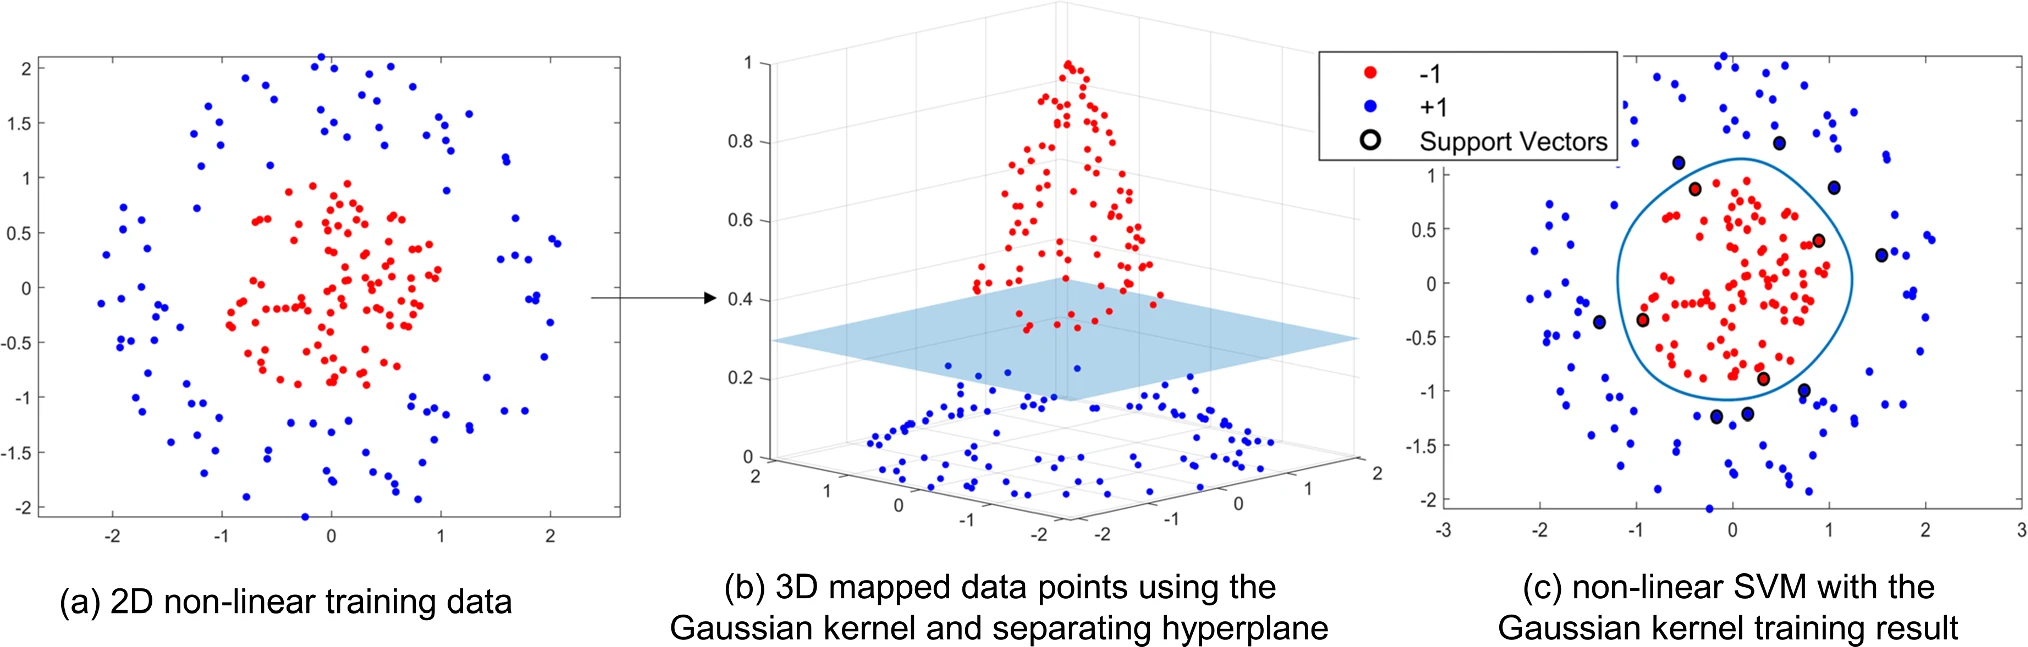
\includegraphics[width=1\linewidth,height=\textheight,keepaspectratio]{extra/svm_kernels.png}

}

\caption{Visualizing Non-Linear Separation with SVM
Kernels\textsuperscript{{[}\citeproc{ref-wang24}{6}{]}}}

\end{figure}%
\end{frame}

\begin{frame}{More Measures of Complexity}
\phantomsection\label{more-measures-of-complexity}
\begin{itemize}
\tightlist
\item
  \textbf{Why?}: VC dimension can be too pessimistic.
\item
  \textbf{Goal}: More nuanced measures, especially for things like
  neural networks.
\end{itemize}

\begin{longtable}[]{@{}
  >{\raggedright\arraybackslash}p{(\linewidth - 4\tabcolsep) * \real{0.2054}}
  >{\raggedright\arraybackslash}p{(\linewidth - 4\tabcolsep) * \real{0.4107}}
  >{\raggedright\arraybackslash}p{(\linewidth - 4\tabcolsep) * \real{0.3839}}@{}}
\caption{Further ways to measure
complexity\textsuperscript{{[}\citeproc{ref-bousquet03}{7}{]}}}\tabularnewline
\toprule\noalign{}
\begin{minipage}[b]{\linewidth}\raggedright
\textbf{Measure}
\end{minipage} & \begin{minipage}[b]{\linewidth}\raggedright
\textbf{Description}
\end{minipage} & \begin{minipage}[b]{\linewidth}\raggedright
\textbf{Key Idea}
\end{minipage} \\
\midrule\noalign{}
\endfirsthead
\toprule\noalign{}
\begin{minipage}[b]{\linewidth}\raggedright
\textbf{Measure}
\end{minipage} & \begin{minipage}[b]{\linewidth}\raggedright
\textbf{Description}
\end{minipage} & \begin{minipage}[b]{\linewidth}\raggedright
\textbf{Key Idea}
\end{minipage} \\
\midrule\noalign{}
\endhead
Covering Numbers & How many ``balls'' cover the hypothesis space? &
Smaller = simpler = tighter bounds \\
\vspace{1pt} Rademacher Complexity & \vspace{1pt} How well can the model
fit random noise? & \vspace{1pt} Lower = less prone to overfitting \\
\bottomrule\noalign{}
\end{longtable}
\end{frame}

\section{Conclusions}\label{conclusions}

\begin{frame}{Key Takeaways I}
\phantomsection\label{key-takeaways-i}
\begin{itemize}
\tightlist
\item
  \textbf{Generalization} is crucial: We want models to work on
  \textbf{unseen data}, not just the training set.
\item
  \textbf{Overfitting} is a risk: More complex models can memorize the
  training data but fail to generalize.
\item
  \textbf{Classical Bounds} highlight the importance of:

  \begin{itemize}
  \tightlist
  \item
    \textbf{Dataset size}: More data leads to better generalization.
  \item
    \textbf{Model complexity}: Simpler models (smaller hypothesis
    spaces) are safer.
  \end{itemize}
\end{itemize}
\end{frame}

\begin{frame}{Key Takeaways II}
\phantomsection\label{key-takeaways-ii}
\begin{itemize}
\tightlist
\item
  \textbf{Advanced Bounds} offer a refined view:

  \begin{itemize}
  \tightlist
  \item
    \textbf{VC Dimension}: Measures a model's ability to shatter data.
    Higher VC dimension means more complexity.
  \item
    \textbf{Distribution-Based}: Leverage data properties for tighter
    bounds.
  \end{itemize}
\item
  \textbf{The Goal}: Balance model expressiveness with the risk of
  overfitting by controlling complexity and leveraging insights from the
  data distribution.
\end{itemize}
\end{frame}

\begin{frame}
\begin{block}{References}
\phantomsection\label{references}
\phantomsection\label{refs}
\begin{CSLReferences}{1}{0}
\footnotesize

\bibitem[\citeproctext]{ref-sklearndiabetes11}
1. Pedregosa F., Varoquaux G., \& et al. (2011). \emph{Scikit-learn:
Machine learning in python, diabetes dataset}.
\url{https://scikit-learn.org/1.5/modules/generated/sklearn.datasets.load_diabetes.html}

\bibitem[\citeproctext]{ref-nakkiran19}
2. Nakkiran P., Kaplun G., \& et al. (2019). \emph{Deep double descent:
Where bigger models and more data hurt}.
\url{https://arxiv.org/abs/1912.02292}

\bibitem[\citeproctext]{ref-mohri12}
3. Mohri M., Rostamizadeh A., \& Talwalkar A. (2012). \emph{Foundations
of machine learning}. MIT Press.

\bibitem[\citeproctext]{ref-samir16}
4. Samir M. (2016). \emph{A gentle introduction to statistical learning
theory}. \url{https://mostafa-samir.github.io/ml-theory-pt2/}.

\bibitem[\citeproctext]{ref-vapnik95}
5. Vapnik V. N. (1995). \emph{The nature of statistical learning
theory}. Springer.

\bibitem[\citeproctext]{ref-wang24}
6. Wang Y., Baek J., \& et al. (2024). Support vector machine guided
reproducing kernel particle method for image-based modeling of
microstructures. \emph{Computational Mechanics}.
\url{https://doi.org/10.1007/s00466-023-02394-9}

\bibitem[\citeproctext]{ref-bousquet03}
7. Bousquet O., Boucheron S., \& Lugosi G. (2003). Introduction to
statistical learning theory. \emph{Advanced Lectures on Machine
Learning}.

\end{CSLReferences}
\end{block}
\end{frame}




\end{document}
